\documentclass[10pt,letterpaper]{article}
\usepackage[margin=1in]{geometry}
\usepackage[T1]{fontenc}
\usepackage{lmodern,microtype,amsmath,amssymb,amsthm,booktabs,array,graphicx,xurl,longtable}
\usepackage[hidelinks]{hyperref}
\usepackage{placeins}
\microtypesetup{protrusion=false}
\setlength{\parskip}{3pt}
\setlength{\parindent}{1em}
\newtheorem{proposition}{Proposition}
\newtheorem{theorem}[proposition]{Theorem}
\newcommand{\R}{\mathbb R}
\newcommand{\F}{\mathcal F}
\newtheorem{lemma}[proposition]{Lemma}
\newcommand{\ind}{\mathbf 1}
\newcommand{\dist}{\operatorname{dist}}
\title{Supplement: Certified Expression Intervals\\under Shared Segmentation Uncertainty}
\author{Arnav Peram\\[2pt]\normalsize Arizona College Preparatory High School\\\normalsize\texttt{arnavperam1@gmail.com}}\date{}
\hypersetup{pdftitle={Supplement: Certified Expression Intervals under Shared Segmentation Uncertainty},pdfauthor={Arnav Peram}}
\begin{document}\maketitle
This supplement gives the continuous realization proofs, atlas construction, count algorithm and experimental details. The mathematical development has two complementary outputs: an exact cut representation for general assignment objectives and coupled boundaries, and a direct hard-budget algorithm for single-boundary point-transcript ribbons. Both use the same canonical minimum-area realization. The experiments evaluate their count certificates on a fixed-seam atlas of the retained observed molecules.

\section{Continuous realization of assignments}\label{sec:continuous}
Use coordinate $t$ along an interface and $x$ across it. Let $m$ ordered boundary graphs $f_a:I\to\R$, $a=0,\ldots,m-1$, divide a compact corridor into $m+1$ cells. Each boundary has a constant slope limit $s_a>0$, a constant band $[\underline b_a,\overline b_a]$, and fixed endpoint values. Adjacent boundaries satisfy
\begin{equation}
0<d_a^{\min}\le f_{a+1}(t)-f_a(t)\le d_a^{\max}.\label{eq:gaps}
\end{equation}
The upper bound may be absent. A rational piecewise-affine reference $f^0$ satisfies these geometric constraints. Exterior rails strictly beyond the bands close the outer cells.

Site $i$ is a rectangle $[x_i^-,x_i^+]\times I_i$ in group $g(i)$; a point is a zero-size rectangle. All sites in a group share cell label $c_g$. Threshold bits $b_{ga}=\ind[c_g\le a]$ satisfy $b_{ga}\le b_{g,a+1}$. For clearance $\rho>0$, requiring the entire site to lie on its assigned side gives
\begin{equation}
 b_{g(i),a}=1\Rightarrow f_a(t)\ge \ell_i=x_i^++\rho,\qquad
 b_{g(i),a}=0\Rightarrow f_a(t)\le u_i=x_i^--\rho\quad(t\in I_i).\label{eq:owners}
\end{equation}
Fixed structural regions have pinned labels and no molecular reward. Nominal RNA locations use point sites. Universal-location regions use~\eqref{eq:owners}; they can make the source assignment inadmissible even though $f^0$ satisfies the geometry.

For a complete assignment $c$, let $\F(c)$ contain its realizing boundaries and define
\begin{equation}
D^\star(c)=\min_{f\in\F(c)}\sum_a\int_I |f_a(t)-f_a^0(t)|\,dt,
\qquad \min\varnothing=+\infty.\label{eq:dstar}
\end{equation}
This is summed interface displacement in the declared coordinates. The later scalar-ribbon construction converts it exactly to physical changed-label area counted once. For arbitrary unary molecular costs $C_g(c_g)$ and $\lambda\ge0$, the penalized objective is $\lambda D^\star(c)+\sum_g C_g(c_g)$; a hard area budget is a different problem.

\subsection{Propagation and exact feasibility}
Give the boundary-index graph an edge $a\to a+1$ of weight $d_a^{\min}$ and, when finite, a reverse edge of weight $-d_a^{\max}$. Let $\Delta_{ab}$ be maximum path weight, with $\Delta_{aa}=0$ and $-\infty$ for no path. Source feasibility excludes positive cycles. Define
\begin{equation}
K_{ab}(r)=\max_v\{\Delta_{av}+\Delta_{vb}-s_v r\},\qquad r\ge0.\label{eq:kernel}
\end{equation}
\begin{lemma}[Heterogeneous propagation]\label{lem:kernel}
Every feasible family obeys $f_b(y)\ge f_a(x)+K_{ab}(|x-y|)$. This is the strongest inequality obtained by finite compositions of the stated slope and same-coordinate difference constraints.
\end{lemma}
\begin{proof}
For any intermediate boundary $v$, transfer from $a$ to $v$ at $x$, travel on $v$ to $y$, and transfer to $b$. This gives each term of~\eqref{eq:kernel}. Conversely choose a boundary of smallest slope rate among the longitudinal portions of a composite path. Its vertical portions before and after that visit are bounded by $\Delta_{av},\Delta_{vb}$. Total absolute longitudinal travel is at least $|x-y|$, at rates at least $s_v$. Hence the path cannot improve that term. The zero-distance case follows from transitive closure.
\end{proof}
The kernels are nonincreasing, $K_{ab}(0)=\Delta_{ab}$, and $K_{ab}(r_1+r_2)\ge K_{av}(r_1)+K_{vb}(r_2)$. A term with rate greater than the destination rate $s_b$ is dominated by its direct-$b$ term; the analogous source statement holds.

A lower requirement $(a,I_i,\ell_i)$ is forbidden if a kernel term $(d,s)$ to any $b$ satisfies $\ell_i+d>\overline b_b$, or $\ell_i+d>f_b^0(e)+s\dist(e,I_i)$ at either endpoint $e$. An upper requirement $(a,I_i,u_i)$ is forbidden if a term of $K_{ba}$ satisfies $u_i-d<\underline b_b$, or $f_b^0(e)>u_i-d+s\dist(e,I_i)$. Add nesting and all fixed-label bits. Finally add
\begin{equation}
b_{g(i),a}\Rightarrow b_{g(j),b}
\quad\text{whenever }\ell_i+K_{ab}(\dist(I_i,I_j))>u_j.\label{eq:imp}
\end{equation}
These are finite unary restrictions and implications; a contradiction means an empty geometric family.

\begin{samepage}
\begin{theorem}[Feasible assignments]\label{thm:feas}
The finite restrictions characterize exactly the complete assignments realizable by the continuous family.
\end{theorem}
\end{samepage}
\begin{proof}
Necessity follows from Lemma~\ref{lem:kernel}; minimum interval distance gives the largest propagated lower requirement. For sufficiency, propagate all active lower requirements, bands and fixed endpoint values into $L_b(t)$, and upper requirements into $U_b(t)$. A lower term is $\ell_i+K_{ab}(\dist(t,I_i))$; an upper term from $a$ is $u_i-K_{ba}(\dist(t,I_i))$. Kernel composition, the triangle inequality, and~\eqref{eq:imp} put every lower term below every upper term. Unary restrictions handle fixed data, so $L_b\le U_b$.
For a directed gap edge $a\to b$ of weight $d$, closure gives $K_{vb}\ge K_{va}+d$ and $K_{av}\ge d+K_{bv}$. Thus $L_b\ge L_a+d$ and $U_a\le U_b-d$. Applying this to reverse edges enforces maximum gaps as well. Dominated rates preserve individual slope limits. Fixed data enforce bands and endpoint equality. Both envelope families therefore satisfy the geometry and realize the selected requirements. Nesting decodes one label per group.
\end{proof}

\subsection{An exact cost function before molecular objectives}
\begin{samepage}
\begin{theorem}[Assignment-wise cost representation]\label{thm:cost}
For rational input, a polynomial-size directed graph with assignment bits $b(c)$, helpers $y$, rational capacities, hard implications and known constant $\kappa$ satisfies
\begin{equation}
\min_y\operatorname{Cut}_{G_D}(b(c),y)+\kappa=D^\star(c)\label{eq:identity}
\end{equation}
for every feasible $c$. Hard-feasible cuts exist exactly for feasible assignments. For arbitrary rational unary molecular costs and rational $\lambda\ge0$, a cut either detects infeasibility or returns an optimum and an attaining rational piecewise-affine boundary.
\end{theorem}
\end{samepage}
\begin{proof}
The family of lower difference inequalities is closed under componentwise minimum and maximum; those operations also preserve each scalar slope bound, band and endpoint. Since $L,U,f^0$ obey the geometry,
\begin{equation}
f_b^*(t)=\min\{U_b(t),\max\{L_b(t),f_b^0(t)\}\}\label{eq:clamp}
\end{equation}
is jointly feasible and satisfies the selected requirements. Every realization has $L_b(t)\le f_b(t)\le U_b(t)$. The clamp is the nearest permitted value to $f_b^0(t)$ at every coordinate, proving simultaneous minimum displacement and~\eqref{eq:dstar}.

An upward displacement is the maximum of nonnegative functions $[\ell_i+d-s\dist(t,I_i)-f_b^0(t)]_+$ activated by bits; downward displacements use complementary bits. Include structural requirements and source-inconsistent RNA requirements. Upward and downward contributions cannot both be positive on a feasible assignment. Split the domain at their affine-piece endpoints, zeros, source knots and pair crossings. On one slab let $h_1\ge\cdots\ge h_k>0$, $h_{k+1}=0$, with $S_j$ the labels in the first $j$ activations. Then
\begin{equation}
\max_{i\text{ active}}h_i=\sum_{j=1}^k(h_j-h_{j+1})\ind[S_j\text{ contains an active bit}].\label{eq:layers}
\end{equation}
Integrate the nonnegative affine differences exactly. An OR term has a standard helper with incoming hard implications and a terminal cost; complementary terms reverse the construction~\cite{kz,kohli}. Repeated labels are included once. Fixed terms are retained in $\kappa$ or forced helpers. Thus minimizing over helpers gives the exact integrated clamp for each fixed $b(c)$, proving~\eqref{eq:identity}. Expand any unary cost as $C_g(m)+\sum_{a<m}[C_g(a)-C_g(a+1)]b_{ga}$ and shift negative terms by a known constant. Rational scaling yields integer capacities. After molecular costs and $\lambda$ are chosen, each numerical hard capacity is set above the resulting total finite capacity. The fixed object is the geometric representation and its logical implications, rather than one numerical big-$M$ for every possible future objective. A cut through a hard arc distinguishes infeasibility;~\eqref{eq:clamp} reconstructs the boundary.
\end{proof}

\paragraph{Graph size versus construction work.}
Let $N$ count all merged RNA and structural rectangles, $G$ groups, and $M_b=O(Nm^2)$ propagated terms on boundary $b$. For one polarity the untruncated terms are $g_i(t)=\alpha_i-s_i\dist(t,I_i)$. Their common reference changes positivity, but not relative cone order. Each pair changes order only constantly many times. An adjacent swap changes one full prefix; starting with $M_b$ prefixes yields $O(M_b^2+M_b)$ distinct activation sets. Simultaneous events may be resolved into adjacent swaps, repeated labels only merge sets, and zero-weight predecessor prefixes support constant-arc helpers. Consequently
\begin{equation}
|V|=O\!\left(Gm+\sum_b(M_b^2+M_b)\right),\quad
|E|=O\!\left(Gm+N^2m^2+\sum_b(M_b^2+M_b)\right).\label{eq:size}
\end{equation}
The auxiliary contribution is $O(N^2m^5)$. Source knots still affect integration, coefficient lengths and reconstruction. Exact intersections, integrals and denominator scaling have polynomial bit complexity. An event integrator updates affected adjacent layers rather than rescanning every layer; on a $J$-knot reference its work is $O((M^2+MJ+J+1)\log(M+J+2))$ rational-arithmetic and bitset operations, given that reference. Queueing adjacent inversions handles multiple crossings; unchanged layer integrals accumulate until the next change. These bounds describe graph construction, with rational operand costs accounted for separately. Arrangement sweeps are established tools~\cite{bentley}.


\section{Physical atlas and exact reference agreement}
The reference is the original labelled raster interpreted as a union of closed pixel squares with disjoint interiors. A positive cell label is eligible when its pixel set is connected and does not meet the crop boundary. Background label zero may participate as the other side of an interface; it is not an additional biological cell. Ineligible cells, crop boundaries and unselected portions of interfaces remain fixed.

For each adjacent eligible label pair, trace shared pixel edges into paths. Split paths at vertices where continuation is ambiguous and into coordinate-monotone runs. Divide long runs at a maximum of 128 unit edges, trim one edge from each end, and retain at least four remaining edges. Rank candidates by length and then by a deterministic label/coordinate ordering. Try ribbon halfwidths $4,2,1,1/2$ pixels in that order. No gene identity, transcript count, count interval or optimization outcome determines this ranking.

Let $s_x,s_y\in\{-1,1\}$ orient a monotone run. Pixel-edge coordinates obey
\[
 t=s_xx+s_yy,\qquad u=s_xx-s_yy.
\]
The run is exactly $u=r(t)$, with slopes $+1$ or $-1$ between its recorded raster vertices. Put $v=u-r(t)$. The inverse physical chart, up to its stored origin, is
\[
 \Phi(t,v)=\frac p2\bigl(s_x(t+r(t)+v),\ s_y(t-r(t)-v)\bigr),
 \qquad |\det D\Phi|=\frac{p^2}{2}.
\]
The pixel size $p$ is read from the source coordinate transformation and retained as an exact rational value. An accepted ribbon has $v\in[-B,B]$, allowed displacement $|h(t)|\le3B/4$, $|h(t)-h(t')|\le|t-t'|$, and zero endpoint displacement. The RNA clearance is $\rho=10^{-6}/p$ in chart coordinates; it separates the two admissible ownership sides numerically. Together these settings define the geometric sensitivity family.

\subsection{Acceptance and nuclear constraints}
Every piece of the left/right half-ribbon is clipped against intersecting native pixels using rational polygon arithmetic. Positive-area intersections must have the declared left/right source labels. Pairwise ribbon interiors must be disjoint. A geometric spatial index selects candidate pairs for the final rational intersection test. RNA coordinates are transformed through the exact chart and their nominal side must agree with the original source mask. A molecule may occur in at most one accepted patch.

A nuclear-mask pixel is labelled by the source \emph{cell} mask at that pixel, rather than by its unrelated nucleus identifier. Clip its square to the ribbon, transform its fragments into $(t,v)$ coordinates, and split at reference-curve knots. Over each projected interval, the maximum required left-side value or minimum right-side value supplies a conservative constant bound. The resulting conservative bound preserves the label of every intersecting nuclear fragment. Structural constraints have zero additional clearance. Encoding structural regions as shifted point/interval constraints cancels the engine's RNA clearance exactly, without adding molecular counts.

An initial extraction pilot omitted nuclei. The final procedure added nuclear constraints and cell--background interfaces before recomputing counts and transferring the fixed rules to the breast crops. The provenance record preserves both stages.

\subsection{Global homeomorphism}
For fixed longitudinal coordinate and any admissible $h$, define
\[
 H_h(t,v)=\begin{cases}
 -B+(v+B)(h(t)+B)/B,&-B\le v\le0,\\
 h(t)+v(B-h(t))/B,&0\le v\le B.
 \end{cases}
\]
Its transverse slopes are strictly positive because $|h|<B$. Both formulas agree at zero, map zero to $h$, and fix $-B,B$. Its inverse is continuous, and $h=0$ at longitudinal endpoints makes the whole boundary trace fixed. Conjugating $(t,v)\mapsto(t,H_h(t,v))$ through $\Phi$ gives a homeomorphism of the closed physical ribbon fixing its boundary. It maps the two source sides to the requested alternatives.

Extend each map by the identity outside its ribbon. Disjoint interiors and fixed traces make the maps agree on intersections. A finite union is therefore a global continuous bijection with the corresponding piecewise inverse. The reference cell topology, connectivity, holes and junction incidences are preserved.

Changed-label area inside one two-label ribbon is exactly
\[
 A(h)=\frac{p^2}{2}\int_I |h(t)|\,dt.
\]
Interiors do not overlap, so changed-label area in the atlas is the sum of these costs, counted once. At source knots the chart is piecewise affine; the finite kink set has zero area. The constant Jacobian makes this conversion exact; other coordinate charts require their corresponding area factor.

\section{Exact assignment-cost function and graph construction}
In an ordered corridor, each boundary has a slope bound, band and endpoint values; adjacent boundaries have constant minimum and optional maximum separations. All finite rational data are binary encoded. The source satisfies the geometric constraints. RNA-location rectangles and pinned structural regions induce lower or upper interval requirements depending on their discrete owner thresholds.

The maximum-path closure $\Delta$ of same-coordinate separation inequalities yields
\[
 K_{ab}(r)=\max_c\{\Delta_{ac}+\Delta_{cb}-s_cr\}.
\]
Every finite sequence of permitted longitudinal and cross-boundary steps is bounded by such a term: choose the least slope on that path, bound its total travel below by the endpoint distance, and its remaining directed weights above by the corresponding closure weights. This gives the complete propagated lower/upper restrictions, including both directions of each finite maximum gap.

The selected lower family $L$, upper family $U$, and reference $f^0$ obey the same geometric difference inequalities. The finite conflict tests imply $L\le U$. Minimum and maximum preserve these inequalities and each scalar slope bound, so
\[
 f_b^*(t)=\min\{U_b(t),\max\{L_b(t),f_b^0(t)\}\}
\]
is a jointly feasible family and is pointwise nearest to the reference. This simultaneous attainment establishes the minimum $D^*(c)$ for each complete assignment.

\subsection{Integrated layers and the helper bound}
In one direction, source-relative excursions are maxima of active flat-top cones. On an analytic interval with ordered positive heights $h_1\ge\cdots\ge h_q>0$, set $h_{q+1}=0$. Their activated maximum equals
\[
 \sum_{j=1}^{q}(h_j-h_{j+1})\,
 \ind[\text{at least one activation among the first }j\text{ occurs}].
\]
Integrate the affine differences exactly. Repeated cones carrying the same molecular bit use that bit once; complementary activations encode the opposite direction. Fixed-positive constraints contribute a mandatory constant or forced helper. Standard implication/OR gadgets then preserve the exact integral for every hard-feasible owner vector. Finite hard capacities exceed the total finite capacity for the requested objective.

For $M$ untruncated flat-top cones, a pair changes order only constantly many times. Starting with $M$ prefixes, each adjacent swap introduces at most one additional prefix. Thus the union contains $O(M^2+M)$ distinct sets. A common reference changes positivity, not cone order. Resolve simultaneous events into adjacent swaps and retain a deterministic tie rule on coincidence intervals. Mapping cone indices to repeated activation labels cannot enlarge the family. A set can use a predecessor prefix plus its last newly added label; retaining zero-weight predecessors keeps the arc count proportional to the number of sets.

If $M_b=O(Nm^2)$ includes all propagated molecular and structural constraints, the graph has
\[
 |V|=O\!\left(Gm+\sum_b(M_b^2+M_b)\right),\quad
 |E|=O\!\left(Gm+N^2m^2+\sum_b(M_b^2+M_b)\right).
\]
The auxiliary contribution is $O(N^2m^5)$. Source knots, intersections and coefficient denominator lengths still affect construction and encoding. Event-driven accumulation can integrate a direction's coefficients in $O((M^2+MJ+J+1)\log(M+J+2))$ rational-arithmetic and bitset operations for a $J$-knot reference. This integration-stage statement is distinct from the final graph-size bound and from total bit complexity. The critical-height algorithm below uses this canonical realization directly to recover every count-specific minimum, including states unavailable to a penalty sweep.

\section{Critical-height count algorithm}
\subsection{Input contract and common mesh}
The count chain specializes the canonical realization to one boundary and one point per free RNA group, with fixed structural regions, a rational piecewise-affine source, slope bounds, bands and endpoints. A free group spanning several locations or an interval would require ownership memory across nodes and lies outside this input contract. Fixed groups may contain many structural rectangles because their labels are known. Group scores are nonnegative integers for each owner, with an integer fixed offset. Atlas, source-observation and saved exact-geometry identities are checked before certification; the count chain checks the raw point-input contract before compilation.

Collect all affine pieces that any canonical realization can select: lower and upper cones for every possible point owner, fixed constraints, bands, endpoints and source. Include all piece endpoints, observation locations and same-boundary intersections in a common mesh. Omit crossings outside the forced envelope only when they cannot be a canonical switch. At every node, candidate heights are function values inside the forced range and outside every observation's clearance gap.

For any complete feasible assignment, its canonical minimizer selects affine pieces between mesh events and crosses the source only at events. Its nodal trapezoidal area is exactly its continuous area. Conversely a feasible candidate path interpolates into a feasible boundary, and its trapezoid upper-bounds that interpolant's area. Retaining the canonical minimizer proves equality of minimum area at \emph{each count}, not equality for every interpolant.

\subsection{Recurrence, sliding minima and reconstruction}
Let $V_j$ be the sorted heights at time $t_j$, $z_j(v)$ the score of points observed at that time, and
\[
 a_j(v)=w_j|v-f^0(t_j)|,\qquad
 w_j=\tfrac12[(t_j-t_{j-1})+(t_{j+1}-t_j)],
\]
with missing endpoint intervals omitted. Each point contributes once. Pinned-group scores enter the initial offset. The least prefix cost satisfies
\[
 F_j(v,q)=a_j(v)+
 \min_{\substack{u\in V_{j-1}\\|u-v|\le s(t_j-t_{j-1})}}
 F_{j-1}(u,q-z_j(v)).
\]
Initialize with first-node cost and score. For each predecessor count, scan candidate heights in increasing order. Insert each permitted predecessor into a monotone deque, discard dominated costs at its back, and discard expired heights at its front. The front gives the least predecessor cost. Both ends of the height-compatibility interval move monotonically, so one node transition takes $O(H_{j-1}+H_j)$ work per count. Backpointers reconstruct a complete owner vector and boundary, which are checked against the original continuous constraints and exactly integrated area.

If the variable score range is $W$, dynamic-programming work is $O((W+1)\sum_jH_j)$ and full backpointer storage has the same order. Value-only rolling storage can be smaller. With $P$ explicit affine pieces, a conservative mesh bound is $O(P^2+P)$ events, at most $O(P)$ heights per event, and $O((W+1)P^3)$ dynamic-programming work. For explicit unit transcripts, $W$ is at most the number of scored molecules. Binary-compressed multiplicities instead give a pseudo-polynomial dependence on $W$. Rational operand lengths, candidate preparation and output serialization remain separate costs.

The implementation raises a resource-limit outcome instead of marking an incomplete spectrum exact. The reference is geometrically feasible but need not realize every point's original owner at zero cost. A positive mandatory-area test exercises that distinction. Single-copy source-feasible queries use the cheaper implication-closure fast path; all multicopy queries in the end-to-end count-chain census use the algorithm above.

\subsection{An explicit unit-molecule penalty gap}
Use source zero on $[0,30]$, slope one, band $[-4,4]$ and clearance $\rho=1/10$. At centers 5, 15 and 25 place respectively 2, 3 and 3 distinct point RNAs. Point $j$ in a cluster has $(t,x)=(\text{center}+j/100,\ h-j/100-\rho)$, with $h=2,3,3$. The slope and clearance force a common owner within each cluster; their leading tents dominate, and clusters have disjoint positive supports. Full owner enumeration gives eight feasible vectors and spectrum
\[
 \{(0,0),(2,4),(3,9),(5,13),(6,18),(8,22)\}
\]
(count, area). At area ten the largest attainable count is three. Every penalty bound is at least four: for $\mu\le1/3$ the count-eight state gives $8-12\mu\ge4$, and for $\mu\ge1/3$ the count-two state gives $2+6\mu\ge4$. At $1/3$ equality holds. All molecules are unit observations at distinct coordinates; no succinct bundle encoding is used. The count chain recovers the unsupported count-three outcome.

\section{Composition, baselines and joint predicates}
For a cell--gene pair with source count $n_0$, each incident patch supplies minimum physical area $S_i(d)$ for count \emph{change} $d$. Use
\[
 S(q)=\min_{d_1+\cdots+d_r=q}\sum_iS_i(d_i),\qquad
 [L,U]=\left[\min_{S(q)\le\delta}(n_0+q),\ 
 \max_{S(q)\le\delta}(n_0+q)\right].
\]
Using changes prevents counting fixed exterior molecules more than once. Zero-relevant patches can stay at their zero-cost source. A minimizing trace yields compatible local witnesses, and the global homeomorphism proves attainability. Restricting any allowed global state to its patches proves the reverse inequality. There is one budget for the complete atlas, not one independent allowance per patch.

The outer baseline lets every individually affordable RNA choose a feasible owner independently. It can combine incompatible changes or overspend the budget; its interval is an outer bound. The additive inner baseline retains exact local feasibility, charges every changed RNA its singleton minimum (including collateral genes), and composes these costs. Under zero-cost source admissibility, this sum upper-bounds shared area, so budget feasibility is an inner approximation. The comparison therefore distinguishes over-permissive independent transfers from over-conservative additive costs.

For co-detection, retain a two-dimensional score and compose vector spectra. Marginal endpoints need not coexist. The tested predicate is $N_{g_1}>0$ and $N_{g_2}>0$, classified as always, never or variable over the budgeted spectrum. The resulting classification describes the stability of observed co-detection under the chosen family.

\section{Data, extraction and complete experimental denominators}
The lung inputs are two 200-micrometre crops of a public Xenium lung-cancer specimen, containing 7,370 retained Q20 measured-gene RNA records. The atlas is extracted directly from the source masks with complete reference-cell containment; it replaces the overlapping corridors of the earlier implementation.

The breast inputs are the two previously acquired source crops in the public workflow artifact identified in the provenance record. The artifact's SHA-256 is \nolinkurl{f53bee7d82a385a320c14a180049e66bf6f60963dda8d7a75574fda90c28febf}. It contains 81,182 retained RNA records and corresponding masks. The source is 10x Genomics' two-field-of-view breast format-test dataset, for which the vendor cautions against biological conclusions. We use these previously available crops to evaluate transfer of the fixed extraction and count-analysis rules.

\begin{table}[ht]\centering
\begin{tabular}{lrrrr}\toprule
 &Lung 1&Lung 2&Breast 1&Breast 2\\\midrule
Retained RNA&5,847&1,523&43,366&37,816\\
Complete reference cells&79&74&253&214\\
Accepted patches&276&268&928&780\\
Editable RNA&627&118&4,789&3,473\\
RNA-bearing patches&190&72&760&628\\
Maximum RNA per patch&19&6&39&33\\
Editable reference edges&7,093&8,728&28,606&24,306\\
All incident reference edges&10,756&12,408&43,331&37,132\\\bottomrule
\end{tabular}
\caption{Complete extraction census. Coverage denominators include incident edges with ineligible neighboring cells. Refer to the machine-readable coverage record for per-cell lengths and fractions.}
\end{table}

The two lung crops have disjoint complete-cell identifiers, as do the two breast crops. Five eligible lung cells have no retained positive gene count and no editable relevant molecule; their rows are implicit zeros in the supplied matrix index. The interval CSV is sparse over every positive-source or editable cell--gene key. Absent entries are zero only within the explicitly recorded panel/observed-gene universe, retained observations and atlas identity. Thus a sparse zero refers to retained observed counts.

All eight budgets $0,0.05,0.1,0.25,0.5,1,2,4\,\mu\mathrm m^2$ are reported. There are 3,304 lung and 22,976 breast cell--gene spectra, yielding 26,432 and 183,808 unique interval rows. One atlas per crop determines every interval and its compatible attaining boundary. Source counts outside editable ribbons remain part of every cell's count.

\subsection{Budget-specific simple-baseline comparisons}
\begin{table}[ht]\centering
\begin{tabular}{lrrrr}\toprule
Area budget&Lung variable&Breast variable&\shortstack{Breast outer\\tightened}&\shortstack{Breast inner\\misses}\\\midrule
0&0&0&0&0\\
0.05&366&3,684&84&11\\
0.1&429&4,414&80&25\\
0.25&524&5,259&61&29\\
0.5&524&5,259&3&3\\
1&524&5,259&0&0\\
2&524&5,259&0&0\\
4&524&5,259&0&0\\\bottomrule
\end{tabular}
\caption{Counts out of 3,304 or 22,976 entries per budget. Lung outer improvements comprise four rows at 0.1; the two lung inner misses occur at 0.1 and 0.25. The differences concentrate at intermediate budgets, where shared area limits the combinations of affordable transfers.}
\end{table}

In breast crop 1, cell 81's LDHB source count is 22. Its minimum attaining count 17 is exactly
\[
 \frac{1977348833190267596699567429}{4085091626228121600000000000}
 \simeq0.48404026497\,\mu\mathrm m^2.
\]
The global trace changes three LDHB molecules through one patch and two through another, plus one collateral KRT8 molecule. A third incident LDHB patch remains unchanged. At budget 0.25 the exact interval is $[19,23]$ versus marginal $[17,23]$; at 0.5 it is $[17,23]$ versus additive-inner $[18,23]$. This example from the complete output shows how the two approximations fail in opposite directions.

\begin{figure}[ht]\centering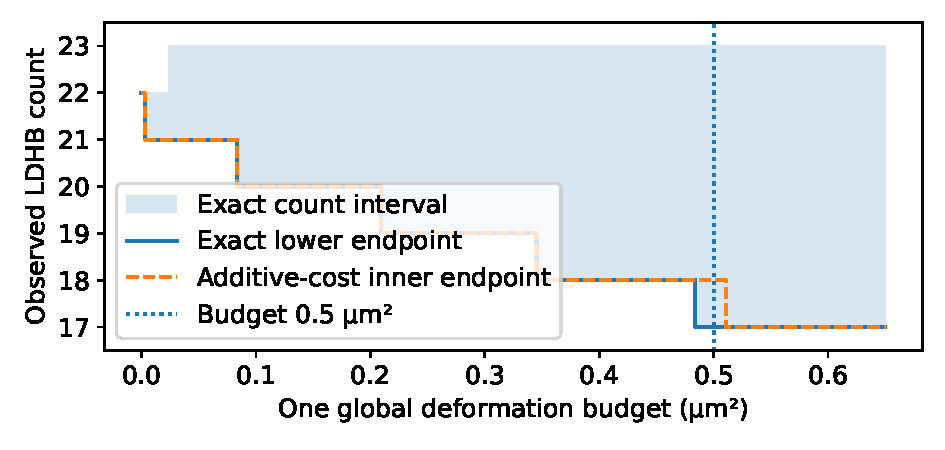
\includegraphics[width=.90\textwidth]{figures/count_curve.pdf}
\caption{The complete LDHB count-spectrum example under unchanged atlas geometry. Step changes follow exact rational minimum areas, rather than interpolation between sampled optimization outputs. The inner comparison can miss an attainable endpoint; the outer comparison can combine individually affordable but jointly over-budget changes.}
\end{figure}


\subsection{Question denominators and endpoint saturation}
On the original eight budgets, 46 lung and 1,026 breast cell--gene questions have marginal width at least two for some budget. Exact geometry tightens four and 203 of these questions, affecting four of 153 lung cells and 139 of 467 breast cells. These question and cell denominators distinguish affected count entries from repeated budget rows. A question is counted once if at least one budget tightens an endpoint.

\begin{table}[ht]\centering
\begin{tabular}{rrrrrrr}\toprule
&\multicolumn{3}{c}{Lung}&\multicolumn{3}{c}{Breast (Xenium)}\\
Area&Variable&Width sum&Endpoints changed&Variable&Width sum&Endpoints changed\\\midrule
0 & 0 & 0 & 0 & 0 & 0 & 0\\
0.05 & 366 & 380 & 366 & 3684 & 4279 & 3684\\
0.1 & 429 & 451 & 70 & 4414 & 5339 & 1028\\
0.25 & 524 & 572 & 120 & 5259 & 6754 & 1350\\
0.5 & 524 & 572 & 0 & 5259 & 6820 & 61\\
1 & 524 & 572 & 0 & 5259 & 6823 & 3\\
2 & 524 & 572 & 0 & 5259 & 6823 & 0\\
4 & 524 & 572 & 0 & 5259 & 6823 & 0\\
\bottomrule\end{tabular}
\caption{Primary eight-budget occupancy, summed widths and number of cell--gene intervals whose endpoints change from the preceding displayed budget. A constant non-singleton total can coexist with further endpoint widening.}
\end{table}


In the original atlas the largest support halfwidth is four chart units. The chart displacement has Euclidean norm $p|h|/\sqrt2$, hence its maximum allowed value is $3pB/(4\sqrt2)\simeq0.4508\,\mu\mathrm m$. This is the geometric displacement cap of the primary atlas. The lung and breast spectra attain their extreme endpoints by areas approximately 0.240525 and 0.573939. Constant non-singleton totals from area 0.25 therefore indicate occupancy saturation earlier than complete endpoint saturation.

\section{Physical-width sensitivity with fixed selection rules}
The prospective analysis record fixes required support halfwidths $r=0.5,1,2,3\,\mu\mathrm m$, the original arc construction, run ordering, endpoint seams, slope one, nuclear constraints and clearance, and the area grid
\[
0,.005,.01,.025,.05,.1,.15,.2,.25,.375,.5,.75,1,2,4,8,16.
\]
The protocol fixes these choices before width-dependent extraction and count calculations on the available inputs. Each run uses $B=\lfloor4\sqrt2r/p\rfloor/4$ and accepts only that width. Rejected patches do not fall back to narrower widths. Longer arcs keep priority and all original coordinate tie rules. Consequently each width defines a separate fixed-seam atlas; the atlases need not be nested.

Every rejected candidate and accepted patch is retained in extraction summaries. Rejection can follow third labels, nuclei inconsistent with required clearance, chart geometry, intersections with earlier selected ribbons, or other declared acceptance conditions. All eligible source cells remain in count denominators, including those without editable patches. Each accepted patch is checked against exact raster-side intersections, all molecular source owners, structural constraints and disjoint interiors.

\begin{table}[ht]\centering
\begin{tabular}{lrrrrr}\toprule
Support&Displacement&\multicolumn{2}{c}{Edge coverage (\%)}&Lung Proseg&Breast nuclear\\
halfwidth&cap ($\mu$m)&Lung&Breast&reach (\%)&reach (\%)\\\midrule
Adaptive&0.451&68.3&65.8&6.6&16.2\\
0.5&0.366&45.1&44.6&4.3&11.2\\
1&0.733&33.8&34.6&5.5&14.8\\
2&1.493&23.5&24.7&4.5&14.6\\
3&2.226&16.9&17.8&3.8&12.2\\
\bottomrule\end{tabular}
\caption{Required physical support halfwidths are rounded down to quarter chart units. The cap is $3pB/(4\sqrt2)$; actual feasibility also depends on other constraints. Reach is the fraction of changed reference counts attainable at any budget, with fixed denominators across families.}\label{tab:reach}
\end{table}


The last endpoint-saturation areas across Adaptive, 0.5, 1, 2 and 3 are, respectively, 0.240525, 0.154063, 1.497699, 3.090472 and 4.878380 for lung; and 0.573939, 0.376462, 1.281168, 5.095884 and 13.782726 for breast. Larger support permits larger movement, but fewer patches fit the same segmentation. The largest local gene multiplicity is 17; the largest patch contains 136 retained molecules. All eight count runs return complete exact spectra.

For like-for-like budget comparisons, the original adaptive-width spectra are also projected onto the 17-budget grid. This uses unchanged rational minima and individually affordable-transfer minima, and every original CSV row matches its earlier value exactly. On this finer grid, 12 of 46 lung and 361 of 1,026 breast questions tighten, versus the primary eight-grid results of 4 of 46 and 203 of 1,026. The finer grid resolves differences over shorter budget ranges in the same underlying spectra. New width columns use the same fine grid.

\begin{table}[ht]\centering
\begin{tabular}{rrrrrr}\toprule
Area ($\mu\mathrm m^2$)&Adaptive&0.5&1&2&3\\\midrule
0 & 0 & 0 & 0 & 0 & 0\\
0.005 & 141 & 78 & 61 & 27 & 24\\
0.01 & 194 & 110 & 84 & 44 & 36\\
0.025 & 287 & 165 & 118 & 57 & 48\\
0.05 & 366 & 227 & 161 & 81 & 72\\
0.1 & 429 & 301 & 224 & 127 & 107\\
0.15 & 484 & 342 & 265 & 160 & 136\\
0.2 & 524 & 342 & 299 & 181 & 162\\
0.25 & 524 & 342 & 320 & 194 & 172\\
0.375 & 524 & 342 & 370 & 226 & 196\\
0.5 & 524 & 342 & 414 & 261 & 218\\
0.75 & 524 & 342 & 427 & 298 & 250\\
1 & 524 & 342 & 427 & 326 & 268\\
2 & 524 & 342 & 427 & 379 & 307\\
4 & 524 & 342 & 427 & 388 & 329\\
8 & 524 & 342 & 427 & 388 & 341\\
16 & 524 & 342 & 427 & 388 & 341\\
\bottomrule\end{tabular}
\caption{Lung: non-singleton intervals on the common 17-budget grid. Column labels after Adaptive are required physical support halfwidths in micrometres. The numbers of question entries for the five families are 3304, 3216, 3298, 3403, 3424.}
\end{table}
\begin{table}[ht]\centering
\begin{tabular}{rrrrrr}\toprule
Area ($\mu\mathrm m^2$)&Adaptive&0.5&1&2&3\\\midrule
0 & 0/0 & 0/0 & 0/0 & 0/0 & 0/0\\
0.005 & 0/0 & 0/0 & 0/0 & 0/0 & 0/0\\
0.01 & 1/3 & 1/2 & 0/2 & 0/0 & 0/0\\
0.025 & 0/8 & 0/2 & 0/2 & 0/0 & 0/0\\
0.05 & 0/14 & 0/2 & 0/2 & 0/0 & 0/0\\
0.1 & 4/26 & 2/8 & 3/9 & 4/7 & 1/4\\
0.15 & 5/35 & 3/14 & 2/15 & 2/12 & 2/9\\
0.2 & 4/46 & 0/14 & 4/24 & 5/17 & 3/10\\
0.25 & 0/46 & 0/14 & 1/27 & 0/18 & 0/11\\
0.375 & 0/46 & 0/14 & 4/31 & 2/19 & 0/11\\
0.5 & 0/46 & 0/14 & 5/38 & 3/26 & 2/17\\
0.75 & 0/46 & 0/14 & 2/40 & 3/28 & 1/17\\
1 & 0/46 & 0/14 & 2/40 & 1/28 & 0/19\\
2 & 0/46 & 0/14 & 0/40 & 2/41 & 1/28\\
4 & 0/46 & 0/14 & 0/40 & 0/41 & 0/31\\
8 & 0/46 & 0/14 & 0/40 & 0/41 & 0/36\\
16 & 0/46 & 0/14 & 0/40 & 0/41 & 0/36\\
\bottomrule\end{tabular}
\caption{Lung: tightened cell--gene questions / questions with marginal width at least two at each budget. Zero over zero denotes no eligible comparison, not a measured zero effect rate. Each question can recur at multiple budgets.}
\end{table}
\begin{table}[ht]\centering
\begin{tabular}{rrrrrr}\toprule
Area ($\mu\mathrm m^2$)&Adaptive&0.5&1&2&3\\\midrule
0 & 0 & 0 & 0 & 0 & 0\\
0.005 & 1431 & 915 & 768 & 514 & 395\\
0.01 & 1927 & 1275 & 1071 & 742 & 557\\
0.025 & 2807 & 1944 & 1594 & 1124 & 834\\
0.05 & 3684 & 2640 & 2165 & 1556 & 1183\\
0.1 & 4414 & 3465 & 2817 & 2049 & 1583\\
0.15 & 4896 & 3852 & 3254 & 2376 & 1808\\
0.2 & 5226 & 3852 & 3563 & 2607 & 2002\\
0.25 & 5259 & 3852 & 3850 & 2830 & 2167\\
0.375 & 5259 & 3852 & 4411 & 3278 & 2508\\
0.5 & 5259 & 3852 & 4770 & 3545 & 2711\\
0.75 & 5259 & 3852 & 4856 & 3951 & 3054\\
1 & 5259 & 3852 & 4856 & 4225 & 3258\\
2 & 5259 & 3852 & 4856 & 4814 & 3670\\
4 & 5259 & 3852 & 4856 & 4876 & 3962\\
8 & 5259 & 3852 & 4856 & 4876 & 4013\\
16 & 5259 & 3852 & 4856 & 4876 & 4013\\
\bottomrule\end{tabular}
\caption{Breast format-test: non-singleton intervals on the common 17-budget grid. Column labels after Adaptive are required physical support halfwidths in micrometres. The numbers of question entries for the five families are 22976, 22538, 23013, 23687, 23772.}
\end{table}
\begin{table}[ht]\centering
\begin{tabular}{rrrrrr}\toprule
Area ($\mu\mathrm m^2$)&Adaptive&0.5&1&2&3\\\midrule
0 & 0/0 & 0/0 & 0/0 & 0/0 & 0/0\\
0.005 & 9/77 & 5/30 & 2/17 & 0/9 & 0/5\\
0.01 & 21/147 & 7/66 & 3/42 & 3/19 & 1/8\\
0.025 & 50/301 & 26/159 & 14/107 & 11/63 & 1/23\\
0.05 & 84/516 & 39/289 & 23/209 & 12/127 & 7/64\\
0.1 & 80/706 & 76/469 & 52/346 & 39/227 & 23/142\\
0.15 & 135/900 & 89/598 & 91/492 & 55/331 & 29/212\\
0.2 & 127/1021 & 24/598 & 82/579 & 46/383 & 29/249\\
0.25 & 61/1026 & 4/598 & 110/674 & 74/452 & 47/291\\
0.375 & 14/1026 & 1/598 & 147/833 & 91/564 & 51/371\\
0.5 & 3/1026 & 0/598 & 148/959 & 91/651 & 56/430\\
0.75 & 0/1026 & 0/598 & 52/990 & 124/780 & 85/528\\
1 & 0/1026 & 0/598 & 8/990 & 125/873 & 86/605\\
2 & 0/1026 & 0/598 & 0/990 & 121/1102 & 83/773\\
4 & 0/1026 & 0/598 & 0/990 & 8/1134 & 67/878\\
8 & 0/1026 & 0/598 & 0/990 & 0/1134 & 2/900\\
16 & 0/1026 & 0/598 & 0/990 & 0/1134 & 0/900\\
\bottomrule\end{tabular}
\caption{Breast format-test: tightened cell--gene questions / questions with marginal width at least two at each budget. Zero over zero denotes no eligible comparison, not a measured zero effect rate. Each question can recur at multiple budgets.}
\end{table}


\begin{figure}[ht]\centering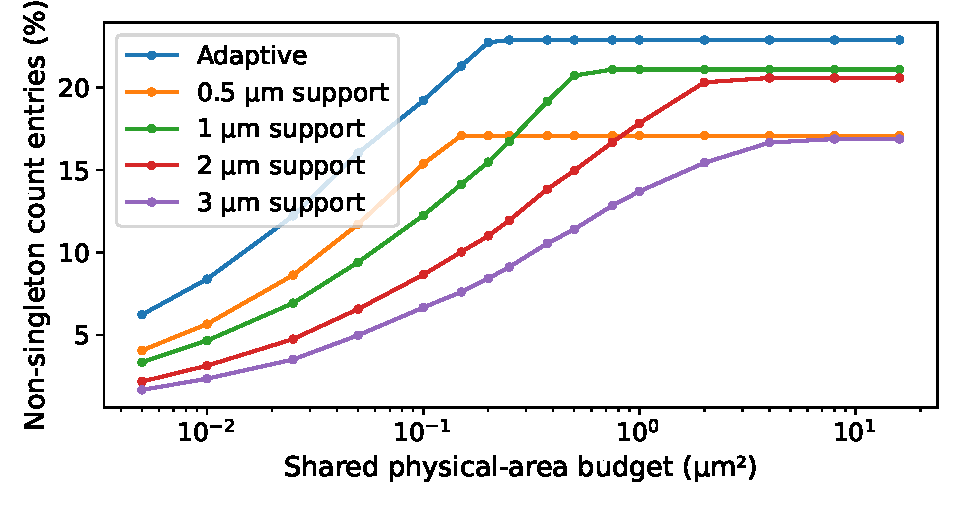
\includegraphics[width=.88\textwidth]{figures/width_budget.pdf}
\caption{Breast interval occupancy under all five separately extracted families. Each denominator is the complete positive-or-editable question set for that family. Width and budget change different aspects of the uncertainty model.}\end{figure}

\FloatBarrier
\section{Reference segmentations and consistent reach denominators}
\subsection{Image-only nuclear reference}
The image-only reference assigns each retained RNA to the nearest labelled nuclear pixel within five physical micrometres, or to background. Nuclear pixels carry their source cell-mask label. RNA coordinates stay fixed. A five-micrometre crop-edge guard excludes points whose nearest nucleus could lie outside the observed crop. This image-only reference provides a deterministic comparison with the expression-informed Proseg output.

\subsection{Proseg executions}
Proseg 3.2.0 was run on the two lung crops. The initial default-factorization run on crop 1 failed during feature selection with an empty-input error. One completed stochastic run per crop used factorization disabled; remaining sampler settings were 200 burn-in iterations, 200 sampling iterations and 50 hill-climb steps, with two requested threads. Diffusion and source reassignment remained enabled. This version exposes no seed argument. Commands, input/output hashes, exclusions and the initial failed log are preserved alongside the raw results. The same two Proseg outputs are compared with every width family.

\begin{table}[ht]\centering\begin{tabular}{lrr}\toprule
Proseg execution quantity&Lung crop 1&Lung crop 2\\\midrule
Input RNA&5,847&1,523\\
Output RNA&5,774&1,482\\
Excluded RNA&73&41\\
Changed source owner&3,242&765\\
Output background/unassigned&2,484&1,335\\
Verified nonzero output-count entries&1,443&67\\\bottomrule\end{tabular}
\caption{Independent ingestion and count-matrix reconstruction of the Proseg executions. Background assignments account for 43.0\% and 90.1\% of output transcripts. The comparison therefore measures the reach of local boundary deformations against substantial assignment changes on clipped crops.}
\end{table}

The check joins exact transcript identifiers, verifies gene names and source assignments, maps Proseg cell labels using the original-cell mapping, and treats the output background flag explicitly. Observed-coordinate serialization residuals are at most 0.000243 and 0.000485 micrometres, respectively. Every saved sparse count entry is reconstructed exactly from the returned assignments. This arithmetic check is independent of the original comparison script; source data and Proseg executions are shared.

\subsection{Countwise reach and assignment-vector exclusion}
All five width families use a common set of comparison keys per reference. Retained transcripts are intersected by exact identifier. Keys whose source count involves an excluded transcript are removed. If a missing transcript is editable in any compared atlas, its gene is also excluded for every candidate destination cell in that patch. These exclusions are applied to every width; all remaining reference and source counts use the same retained observations. Thus denominators remain fixed across widths, and missing Proseg records or crop-edge nuclear exclusions cannot masquerade as changes.

The common comparison has 2,798 changed lung Proseg count keys, 1,114 changed lung nuclear keys and 10,965 changed breast nuclear keys. These differ from the original adaptive-only nuclear comparison (1,128 and 11,151 changed keys) because the new exclusion guard covers the union of editable observations over every width. Included/excluded keys and reasons are supplied explicitly.

At each budget a reference count is attainable exactly when its count-specific minimum area is within budget. Unbounded-budget reach tests membership in the entire finite count spectrum. The main paper's reach table gives the latter results; all 17 finite budgets are exported. The complete reference assignment vector is ruled out in each crop at every width by at least one changed fixed RNA or unavailable destination. This exclusion is stronger than merely observing that some count misses its interval. Conversely, countwise inclusion cannot establish a jointly realizable reference matrix.

A widening ribbon need not improve aggregate reach because its required support removes other patches. The width study separates the displacement available inside accepted ribbons from the extent of tissue covered by those ribbons.

\subsection{Co-detection in the primary atlas}
The three tested pairs are EPCAM/PTPRC, EPCAM/CD3D and EPCAM/PECAM1. The primary atlas contains 150 lung and 1,148 breast cell/pair questions, each evaluated at eight budgets. Table~\ref{tab:codetection} separates persistent co-detection from source positives that can be removed and source negatives that can become positive. The classifications reached by area $0.25\,\mu\mathrm m^2$ persist through the largest tested area of $4\,\mu\mathrm m^2$. The vector spectra and marginal intervals give the same classifications on these inputs.

\begin{table}[ht]\centering
\begin{tabular}{llrrrr}\toprule
 &Pair&\shortstack{Source\\positive}&Removable&Persistent&\shortstack{Newly\\possible}\\\midrule
Lung&EPCAM/PTPRC&7&2&5&0\\
 &EPCAM/CD3D&3&0&3&0\\
 &EPCAM/PECAM1&3&0&3&0\\
Breast&EPCAM/PTPRC&48&2&46&4\\
 &EPCAM/CD3D&0&0&0&0\\
 &EPCAM/PECAM1&47&5&42&3\\\bottomrule
\end{tabular}
\caption{Co-detection at area $0.25\,\mu\mathrm m^2$ in the primary atlas. Removable and persistent counts partition the source positives; newly possible counts describe source-negative cells. Each classification concerns joint positivity of the indicated pair.}\label{tab:codetection}
\end{table}

\paragraph{Interpretation.}
These experiments quantify sensitivity within the stated geometric family. Fixed seams and junctions restrict its reach, and its width and budget parameters have yet to be anatomically calibrated. The two crops per tissue and repeated budget queries provide computational replication, rather than an independent donor cohort. The breast crop provenance limits biological interpretation. The nuclear and Proseg comparisons measure alternative assignments; they provide neither transcript-level truth nor a segmentation-accuracy benchmark. Likewise, stable or removable co-detection alone does not identify a cell state, doublet or leakage.

\FloatBarrier
\section{Validation and resource measurements}
The independent scalar reference uses Fraction arithmetic but imports none of the production implication, envelope, integrated-layer, min-cut or count-chain routines. It recomputes the minimum for every target assignment, then uses Cartesian products for global truth. Inputs and their extraction remain shared. Continuous witnesses have a further direct slope, band, owner, nuclear and rational-area check.

\begin{table}[ht]\centering
\begin{tabular}{lrr}\toprule
Check&Lung&Breast crops (Xenium)\\\midrule
Independent local gene spectra&706&7,068\\
Target binary assignments&1,498&17,542\\
Local witness records&1,101&11,594\\
Global spectra&3,304&22,976\\
Cartesian tuples&3,905&32,730\\
Global attaining count witnesses&3,876&29,799\\
Unique budget intervals&26,432&183,808\\
Exact half-ribbon/pixel checks&31,642&105,824\\
Relevant ribbon-pair checks&491&1,602\\
Nuclear pixel fragments&6,609&42,732\\\bottomrule
\end{tabular}
\caption{Exact validation of the primary atlas: all comparisons agree and every attaining witness satisfies the continuous constraints.}
\end{table}

The count-chain test suite additionally compares 201 scalar spectra on 100 generated systems, tests 80 nonflat models against 1,644 exhaustive assignments, verifies positive mandatory deformation and rejection of free interval-valued RNA, and checks the explicit eight-unit gap. All 944 multicopy local gene questions from both data collections agree with independently enumerated spectra. A full hybrid reanalysis uses the chain for all multicopy genes and closure for single-copy genes; every global minimum area and every interval CSV row matches the separately checked enumerated calculation. The transversely monotone gluing map passes inverse, trace, chart roundtrip and independent polygon-area checks.

\subsection{Width-study checks}
All eight width analyses completed, giving 106,351 global spectra and 1,807,967 interval rows. Local attaining boundaries were checked in continuous coordinates during computation. A separate composition routine reconstructed every global spectrum and checked 131,376 attaining traces, including source counts, local contribution signs, total area and unique transcript support. Every interval row was then recomputed from its exact spectrum and compared with its marginal outer bound.

Independent scalar enumeration checks a deterministic hash-selected sample of up to 32 multicopy questions per setting, restricted to two--six target copies: 246 spectra and 1,628 target assignments in total. All sampled minima agree within the 15-second per-query limit. The new forced-owner preprocessing is additionally tested on 80 generated models: 160 spectra, 773 target assignments and 287 witnesses agree among unpruned chain, pruned chain and separate scalar enumeration. Preprocessing substitutes only hard-implication consequences; it changes no feasible owner vector.

A single process per width computes its complete spectra with a 60-second local chain allowance. Timings for these simultaneous runs record their computational cost; the sequential repeated scaling experiment below measures runtime under a controlled schedule. All computations use the same ingested observations, masks and prepared atlas geometry.

\subsection{Count-chain scaling}
The fixed constructed family has flat source, slope one, equal flipped height $h=1/4$, site spacing $d=1/10$, clearance $1/1000$, a containing band and endpoints outside all tents. The minimum for $k\ge1$ changes is
\[
 A_k=h^2+(k-1)(hd-d^2/4),\qquad A_0=0,
\]
attained by $k$ consecutive sites. For arbitrary selected sites, each additional separation contributes at least the adjacent-site area increment, which proves the lower bound. The closed-form spectrum provides an exact reference for measuring the general count chain as input size grows.

\begin{table}[ht]\centering
\begin{tabular}{rrrrrr}\toprule
RNA&Count levels&Mesh nodes&Height candidates&Visited states&Median total(s)\\\midrule
16&17&111&1,154&8,112&0.465\\
32&33&207&2,370&35,104&1.574\\
64&65&399&4,802&147,456&7.138\\
128&129&783&9,666&605,632&42.206\\\bottomrule
\end{tabular}
\caption{Three fresh sequential processes per size. Total includes preparation, dynamic programming, all witness reconstruction and continuous checks. No limit is reached.}
\end{table}

The 128-RNA totals range from 40.189 to 42.704 seconds. Median mesh compilation is approximately 2.033 seconds and dynamic programming plus all witness output/checking approximately 40.152 seconds; separate medians need not sum exactly. The tested limits are 300,000 retained candidate heights, one million visited states, 60 seconds for preparation, 90 seconds for dynamic programming, and 160 seconds for a complete process. Requested single-thread environment variables are recorded, but the arithmetic is Python integer/Fraction work. Peak whole-process RSS at the largest size is approximately 205 MiB and includes imports. Raw process records contain the exact environment and wall/memory measurements.

\FloatBarrier
\section{Reproduction, data rights and assistance}
The prepared-input exact workflow uses Python's standard library. Geometry extraction, raster reference analysis and plotting additionally use the declared analysis dependencies. The main commands are:
\begin{verbatim}
python atlas_cli.py verify-manifest
python release/restore_results.py
python atlas_cli.py showcase --output run/showcase.json
python atlas_cli.py validate
python analysis/reach/audit_proseg.py
python analysis/reach/check_outputs.py
python analysis/reach/report.py
\end{verbatim}
The README lists separate commands for each main table and figure, the original full count computations and each width-specific recomputation. Compressed result files are restored only after their stored and expanded checksums agree. Source packages retain all original and new spectra, witnesses, comparison keys, Proseg records, selection rules and reference masks. The archive records both exact numerical checks and the environments used for runtime measurements.

The GeoCert software is released under the MIT License. Original 10x data retain CC BY 4.0 attribution and the breast format-test limitation. Proseg retains its upstream rights; its executable is not redistributed. Source code, inputs and exact results for the 1.1.0 companion are publicly archived at \url{https://github.com/arnavperam/geocert/tree/6581f628a5ac8fb83629f9e0dee0ffa4d685375d/recomb2027-atlas}. This immutable source revision is distinguished from the separately rebuilt PDF artifacts in the release record.

Generative AI assisted mathematical development, code, experiments, checking and drafting. The author is responsible for the submitted claims and their explanation. The validation sections specify the independent calculations and their shared inputs.
\begin{thebibliography}{9}
\bibitem{kz} V. Kolmogorov and R. Zabih. What energy functions can be minimized via graph cuts? \emph{IEEE TPAMI} 26(2):147--159, 2004. doi:10.1109/TPAMI.2004.1262177.
\bibitem{kohli} P. Kohli, L. Ladick\'y and P. H. S. Torr. Robust higher order potentials for enforcing label consistency. \emph{International Journal of Computer Vision} 82:302--324, 2009. doi:10.1007/s11263-008-0202-0.
\bibitem{bentley} J. L. Bentley and T. A. Ottmann. Algorithms for reporting and counting geometric intersections. \emph{IEEE Transactions on Computers} C-28(9):643--647, 1979. doi:10.1109/TC.1979.1675432.

\bibitem{biologicalbreast} 10x Genomics. FFPE Human Breast with Pre-designed Panel. Xenium Onboard Analysis 1.0.2; ductal and lobular carcinoma donors. CC BY 4.0. \url{https://www.10xgenomics.com/datasets/ffpe-human-breast-with-pre-designed-panel-1-standard}. Accessed 31 October 2026.
\end{thebibliography}

\end{document}
